\chapter{General source distributions}
% draw cartoons, remember W is wiener, reread ICFM, give examples, customisable serving of information, write terms used throughout papers, find terms that need explanation, UNet and Transformer and optimisation in appendix, parametric function is non linear, 
$p_1(\rmY)$?
\section{Preliminaries on noise suppression with diffusion models}
\[
\bar\rmX = \rmX\ast\mH + \rmZ
\]
Instead of a variance preserving SDE, consider a variance exploding SDE
\[
\dd\rmX=\gamma(\bar\rmX - \rmX_u)\dd u + \sqrt{ck^{2u}}\dd\rmW_t.
\]
\[
\rmM(\bar\rmX,\rmX,u;\gamma) = e^{-\gamma u}\rmX + (1- e^{-\gamma u})\bar\rmX \qquad \tSigma(u;\gamma,c,k) = \frac{c(k^{2u}-e^{-2\gamma u})}{2(\gamma + \log k)}\tI
\]
\section{Schr\"odinger bridge}\label{sec:schr}
\begin{figure}
    \centering
    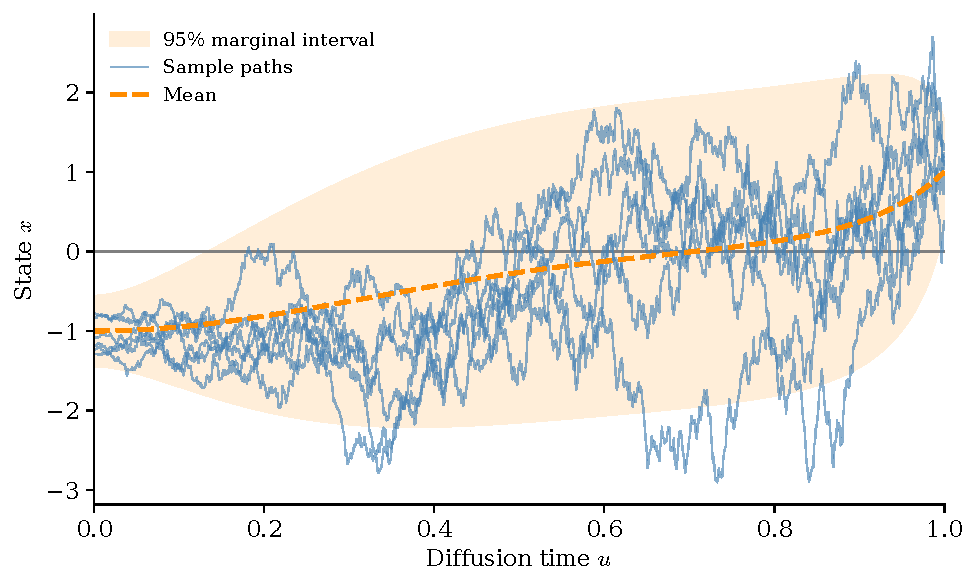
\includegraphics[width=1\linewidth]{plots/schrodinger_bridge_sde.pdf}
    \caption{Enter Caption}
    \label{fig:schrodinger_bridge}
\end{figure}
SB allows a Brownian path between data boundaries.
\[
\min _{p \in \mathcal{P}_{\left[0, 1\right]}} D_{\text{KL}}(p, p_{ref}) \quad s.t. \quad p_0=p_x, p_1=p_y
\]
\[
\dd\rmX = \left[\mF + g^2(u)\nabla\log\mPsi_u\right]\dd u + g(u)\dd \rmW_u
\]
\[
\dd\rmX = \left[\mF - g^2(u)\nabla\log\hat\mPsi_u\right]\dd u + g(u)\dd \hat\rmW_u
\]
Where $\mPsi$ and $\hat\mPsi$ are optimal forward and reverse probability flows. The coupled distribution then becomes $p_u=\mPsi\hat\mPsi$.
Consider a purely variance-exploding reference process
\[
\dd \rmX = \bm 0 \dd u + \sqrt{ck^{2u}}\dd\rmW_u
\]
\[
\sigma_u^2 = \frac{c(k^{2u}-1)}{2 \log k},
\]
\[
  \label{eq:sb_mean_variance}
  \rmM_u(\rmX_0, \rmY) = \left(1 - \frac{\sigma_u^2}{\sigma_1^2}\right) \rmX_0 + \frac{\sigma_u^2}{\sigma_1^2} \rmY ,
\]
\[
\tSigma(u) = \sigma_u^2 \left(1 - \frac{\sigma_u^2}{\sigma_1^2}\right)\tI, 
\]


The loss is data prediction given a path sample
\[
\mS_\theta(\rmX_u|\bar\rmX,\ru)-\rmX_0
\]

\section{Notes on the SB design space}\label{sec:sbsv}
The mean $\rmM$ tends to linear interpolation as $k\rightarrow1$. The variance $\tSigma$ is $0$ at the boundaries and increases. This dynamic movement can make deep learning more difficult. Given that this variance is artificial, it is important to determine the benefits of this noise.

\section{Conditional flow matching}\label{sec:icfm}
\begin{figure}
    \centering
    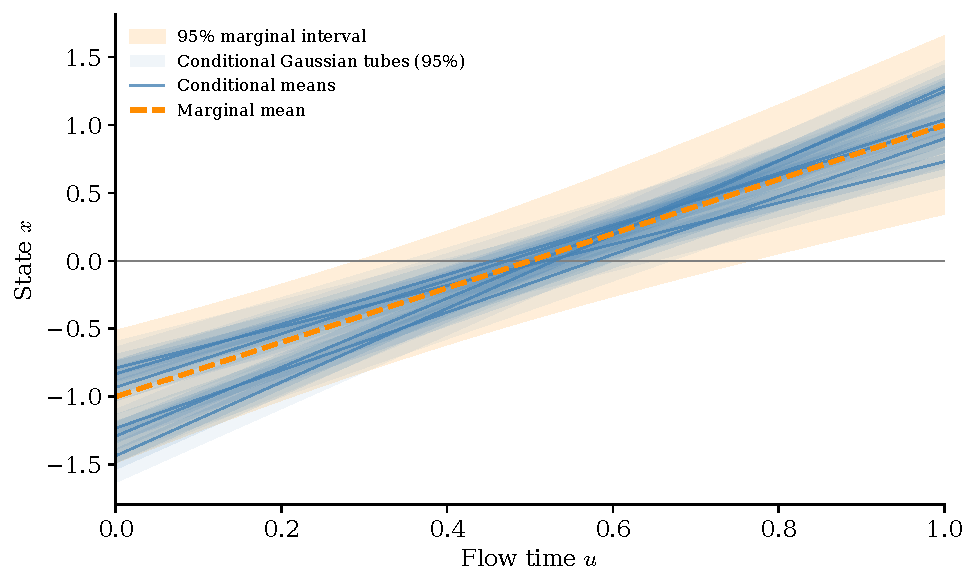
\includegraphics[width=1\linewidth]{plots/independent_conditional_flow_matching.pdf}
    \caption{Enter Caption}
    \label{fig:conditional_flow_matching}
\end{figure}
A less obvious yet simpler approach is a linearly interpolating mean and constant variance.
\[
\dd \rmX=\bar\rmX - \rmX \dd u
\]
\[
\rmM(\rmX_0,\rmY,u) = u\rmY + (1-u)\rmX_0 \quad \sigma(u)^2=c
\label{eq:icfm_mean_variance}
\]
\[
\mS_\theta(\rmX_u|\bar\rmX,\ru)-(\rmX_0 -\bar\rmX)
\]

\section{Inference schemes}
The ODE sampler is defined as
\[
\mX_{u_{n-1}}=a_n\mX_{u_n} + b_n\mS_\theta(\mX_{u_n},\bar\mX,u_n) + c_n\bar\mX
\]
Direct data prediction with data prediction loss is
\[
\mX_0=\mS_\theta(\bar\mX, \bar\mX,1)
\]
and for flow-matching loss
\[
\mX_0=\mS_\theta(\bar\mX, \bar\mX,1) + \bar\mX
\]
